%%%%%%%%%%%%%%%%%%%%%%%%%%%%%%%%%%%%%%%%%%%%%%%%%%%%%%%%%
%%%%%%%%%%%%%%%%%%%author:rickymf4%%%%%%%%%%%%%%%%%%%%%%%
%%%%%%%%%%%%%%%%%%%%%%%%%%%%%%%%%%%%%%%%%%%%%%%%%%%%%%%%%
\chapter{实战方法}
\label{chap:11}

成功地应用深度学习技术远远不仅仅需要知道有哪些算法和这些算法的原理。一个好的机器学习实践者亦需要知道如何针对特定的应用选择算法,如何监控实验并对获得的反馈做出回应,从而优化该机器学习系统。在机器学习系统的日常开发中,实践者们需要决定是否需要搜集更多的数据,是增加还是减少模型的容量,是加上还是去掉规则化特征,是改进模型的优化,还是改进模型中的近似推理,亦或是对模型的实现程序进行调试。所有这些操作都是非常耗时的尝试,所以能够确定正确的行动方针是很重要的,而不是盲目猜测它。

这本书的大部分内容是关于各种机器学习模型、训练算法,和目标函数。这可能会造成这样的印象:成为机器学习专家最重要的本领是要了解各种机器学习技术并擅长不同类型的数学。 然而在实践中,正确地使用一个常见的算法比草率地使用一个晦涩的算法要好。算法的正确应用取决于掌握一些相当简单的方法。本章节中许多建议改编自\cite{Ng ( 2015 )}.

我们建议如下的实际设计过程:
\begin{itemize}
\item 确定您的目标 - 要使用的误度量和相应的目标价值。这些目标和误差度量应该由应用要解决的问题来驱动。
\item 尽快建立一个可以工作的端到端的流水线,包括适当估计它的性能指标。
\item 较好地给系统装上仪表来确定其性能瓶颈。诊断哪些组件的性能低于预期,以及是否是由于过度拟合、欠拟合,或数据或程序中存在着缺陷。
\item 基于来自仪表中特定的发现,重复地进行增量变更,如收集新数据,调整超参或更改算法。
\end{itemize}

我们将采用街景地址号码翻译系统作为一个运行的例子 (\cite{ Goodfellow et al. , 2014d })。 这个应用的目的是将建筑添加到谷歌地图中。街景车对建筑进行拍摄并记录照片对应的GPS坐标。通过卷积网络来识别每张照片中的地址号码,使得谷歌地图数据库可以将该地址加入到正确的位置上。关于如何开发这个商业应用程序的故事给出了如何遵循我们倡导的设计方法的例子。我们现在来描述这个过程中的每个步骤。

\section{性能指标}

确定目标(根据将采用的错误率指标)是必要的第一步,因为你的错误率指标将指导你以后的所有操作。你还应该知道你想要什么级别的性能。

请记住,对于大多数应用,不可能实现绝对零错误率。即使你有无限训练数据,并且可以恢复真实的概率分布,而贝叶斯误差定义了你可以希望实现的最小错误率。这是因为你的输入特征可能不包含有关输出变量的完整信息,或者因为系统可能是内在随机的。你也将受限于有限数量的训练数据。

由于各种原因,训练数据的量被限制了。当你的目标是构建一个一流的实际的产品或服务时,您通常可以收集更多数据,但必须确定进一步减少错误率的价值,并将其与收集更多数据的成本进行权衡。数据收集可能需要时间、金钱或使人遭受痛苦(例如,如果您的数据收集过程涉及侵入性的医学测试)。 而当你的目标是回答在固定的基准上哪个算法的表现更好时,通常是不允许收集更多数据作为基准的训练集的。

如何给性能水平确定一个合理的期望?通常,在做学术时,我们基于以前发布的基准测试结果,可以做一些错误率的估计。而在做实际项目时,我们考虑的错误率是要让我们的应用是安全的,成本效益的,或是吸引消费者的。一旦确定了实际期望的错误率,那么为了达到此错误率将指导你的设计决策。

除了性能指标的目标值之外的另一个重要考虑是选择使用哪个指标。可以使用几种不同的性能指标来测量一个完整的包含各种机器学习组件的应用的有效性。这些性能指标通常不同于用于训练模型的代价函数。 如第5.1.2节所述,我们通常测量系统的准确率或错误率。

然而,许多应用需要更高级的指标。

有时一种错误的代价会比另一种更高。例如,电子邮件垃圾检测系统可能产生两种错误:错误地将合法的邮件分类为垃圾邮件,以及错误地允许垃圾邮件在收件箱中显示。

阻止合法消息比允许可疑消息通过更糟糕。 我们不是测量垃圾邮件分类器的错误率,我们可能希望用某种形式来衡量总体代价,认为阻止合法邮件的代价高于允许垃圾邮件。

有时我们想要训练一个二元分类器,用于检测一些异常事件。例如,我们将要为一个罕见的疾病设计一个医学测试。假设每百万人中只有一人患有这种疾病。我们通过简单地将分类器结果固定为无疾病,可以很容易地实现99.9999%的检测精度。显然,用准确性来表征这种系统的性能的是不行的。 解决这个问题的一种方法是改为采用精度和召回(ure precision and recall)的统计方法。精度是模型的检测结果中正确的比例,而召回是真实事件被模型检测到的比例。当一个检测器说没有人患这种疾病时将有完美的精度,但召回是零。当一个检测器说每个人都有疾病时将实现完全召回,但精度等于患有该疾病的人的百分比(在我们的例子中,一百万人中有一人的比例是0.0001%)。当使用精度和召回时,我们通常绘制PR曲线,y轴表示精度,x轴上表示召回。当待检测的事件发生时,分类器将输出较高的分数。 例如,一个检测疾病的前馈网络的输出$\hat{y} = P(y=1|\Vx)$,表示医疗结果具有特征x的人的患病概率。当该输出概率分数大于某个阈值时,则认为检测到了。通过改变阈值,我们可以权衡在某召回下的精度。在许多情况下,我们希望用单个数字而不是曲线来总结分类器的性能。为此,我们将精度p和召回r转换为一个F分数:

\begin{equation}
        F = \frac{2pr}{p+r}.
\end{equation}

另一个方法是统计位于PR曲线下方的总面积。

在一些应用中,机器学习系统可以拒绝做决定。当机器学习算法可以估计一个决策的可信度时这是有用的,特别是如果错误的决策可能带来危害并且操作人员能够偶尔接管的话。街景翻译系统就是这样一个例子。 它的任务是从照片中翻译地址号码,以便将拍摄照片的位置与地图中的正确地址相关联。因为如果地图不准确,地图的价值会大大降低,所以只有在翻译正确的情况下才添加地址非常重要。如果机器学习系统比人类更难获得正确的翻译,那么最好的办法就是让人来替代。当然,如果机器学习系统能够大大减少运营人员必须处理的照片数量,那么它是有用的。在这种情况下使用覆盖率来作为性能指标。覆盖率是机器学习系统能产生响应的样本的比率。 可以将覆盖率和准确率进行权衡。 如果我们决绝了所有样本,则能获得100\%的准确率,但覆盖率减少到0\%。对于街景翻译这个任务,目标是在保持95\%的覆盖率下达到人类水平的翻译准确率。在这个任务上,人类水平为98\%。

还有可能是其它指标。 例如,我们可以衡量点击率,收集用户满意度调查等。许多专业应用领域也有应用特定的标准。

重要的是确定要先提高哪个性能指标,然后集中精力提高这个指标。没有明确的目标,很难判断机器学习系统的优化是否取得进展。


\section{默认基准模型}

选择性能指标和目标后,下一步,对于任何的实际应用都是要尽快建立一个合理的端到端系统。 在本节中,我们提供了在各种情况下用哪个算法作为第一个基准方法建议。 请记住,深度学习研究是进展很快的,所以更好的默认算法可能在写完后很快就能用。

根据你的问题的复杂性,你甚至可能不想使用深度学习。如果你的问题可以通过正确地选择一些线性权重就能解决,你可能从一个简单统计模型开始做,如逻辑回归。

如果你知道你的问题属于“AI-完全的”类别,如物体识别,语音识别,机器翻译等等,那么你很可能通过一个恰当的深度学习模型来做出比较好的效果。

首先,根据你的数据的结构,选择一个类型的模型。如果你想做有监督学习,而且有固定大小的向量作为输入,那么使用带全连接层的前馈网络。如果已知输入的拓扑结构(例如,输入是一幅图像),那么使用卷积网络。在这些情况下,你应该从使用一些分段线性单元(ReLUs 或其推广如Leaky ReLUs,PreLus和MAXOUT)开始。如果你的输入或输出是一个序列,那么使用门控递归神经网络(LSTM或GRU)。

优化算法的合理选择是带动量的随机梯度下降法(SGD),加上带衰减的学习率(流行的衰减方法在不同的问题上表现有好有坏,包括:线性地衰减到一个固定的最小值,指数衰减,或每次遇到验证错误率趋于平稳时将学习效率降低2到10倍)。另一个非常合理的选择是Adam方法。批量归一化对优化性能有很大的影响,尤其是卷积网络和带sigmoidal 的非线性的网络。虽然你刚开始的第一个基线不用批量归一化是合理的,但如果优化似乎是有问题的,应该马上使用它。

除非你的训练集包含了数千万的例子或更多,否则你应该从开始就引入一些轻度的正规化。及早停止普遍被使用。Dropout是一种不错的正则化方法,它易于实现,并与许多模型和训练算法兼容。批量归一化也往往能降低泛化误差,而不用dropout,这是因为在用于规范化每个变量的统计估计中存在噪声。 

如果你的任务和另一个被广泛研究的任务相似的话,你可以先拷贝那些已经被证明在先前研究任务上表现最好的模型和算法,从而获得比较好的结果。您甚至可以从该任务复制一个训练好的模型。例如,一个是常见的做法是使用基于在ImageNet上训练得到的卷积网络的特征,来解决其他计算机视觉任务(\cite{Girshick,2015})。

一个常见的问题是,是否要使用无监督学习,我们会在第三部分进一步介绍。这是和一些特定领域的有关的。有一些领域,如自然语言处理,都大大受益于无监督学习技术,如学习无监督词嵌入。在其他领域,如计算机视觉,目前的无监督学习技术没有优势,除了基于少量标记样本的半监督的学习(\cite{Kingma等,2014;Rasmus等,2015})。如果无监督学习对你的应用重要时,那么你可以引入它作为你第一个端到端学习的基线。否则,只有当你想解决的任务是无监督的时候,你才用无监督学习。还有,如果你发现你的初始基线过拟合了,你总是可以在后期尝试引入无监督学习。


\section{确定是否收集更多的数据}

在建立了第一个端到端的系统之后,接下来便是测量我们的算法性能,并确定如何改进它。 许多机器学习新手试图通过尝试许多不同的算法来进行改进。 然而,收集更多的数据往往要比改进学习算法更有效。

如何决定是否收集更多的数据? 首先,确定在训练集上的性能是否是可接受的。 如果在训练集上的性能差,那么学习算法并没有利用已有的训练数据,因此没有理由收集更多数据。 相反,得尝试通过添加更多的层或向每个层中添加更多隐藏单元来增加模型的大小。 此外,还得尝试改进学习算法,例如通过调整学习率等超参。如果你用的是大模型,并且对其进行了精心的调整优化,却不能很好地工作,则可能是训练数据质量的问题。 数据可能含有太多噪声,或可能不包括待预测的目标输出的所需的正确输入。这时建议你从头开始,收集更干净的数据或收集更丰富的特征集合。

如果在训练集上的性能可接受,那么对测试集上的性能进行测试。如果测试集上的性能也是可接受的,那么没有什么可以做的了。如果测试集上的性能比训练集上的性能糟糕得多,那么最有效的解决方案之一便是收集更多的数据。要考虑的关键因素是收集更多数据的成本和可行性,通过其他方式降低测试集错误率的成本和可行性,以及预期能显着提高测试集性能的所需的数据量。在拥有数百万或数十亿用户的大型互联网公司,收集大型数据集是可行的,这样做的费用可能远低于其他替代方案,因此答案几乎总是收集更多的训练数据。例如,构建大规模的标记数据集是解决目标识别的最重要的因素之一。而在其他情况下,例如医疗应用,收集更多数据可能是昂贵的或不可行的。一个简单的替代收集更多数据的方法是通过调整超参(例如权重衰减系数)或通过添加正则化策略(例如dropout)来减小模型的大小或改进正则化。如果您发现即使调整正则化超参后,训练和测试性能之间的差距仍然不可接受,那么建议你收集更多的数据。

在决定要收集更多数据时,还需要决定收集多少。我们可以绘制训练集大小和泛化误差之间的关系曲线,如图\ref{fig:5_1}所示。 通过外推这样曲线,可以预测要达到某个性能水平所需要的额外训练数据量。通常,添加相对总量很小的一部分样本数量不会对泛化错误产生显着影响。 因此建议你以对数标量来设置训练集的大小进行实验,例如使相邻两次实验之间的数据量加倍。

如果收集更多的数据是不可行的,唯一一个其它的方法是改进学习算法本身来改进泛化误差。这变成是一个研究领域,而不是一个单单给应用实践者一些建议的范畴。

\section{超参的选择}

大多数的深度学习算法有许多超参,它们控制着算法行为的诸多方面。有的超参影响算法运行的时间和内存的消耗,有的则影响着通过训练过程来复原模型的质量和对新的输入推断出正确结果的能力。

有两种选择超参的基本方法:即人工选择和自动选择。人工选择超参需要理解超参的作用以及是如何帮助机器学习模型达到好的泛化的。自动选择超参可以大大降低对这些思想理解的需要,但它们往往有更大计算代价。


\subsection{手动超参调整}

为了手动设置超参,你必须知道超参、训练误差、泛化误差和计算资源(内存和运行时间)之间的关系。这着这意味着建立一个坚实的基础,是在第5章中提到的关于学习算法有效容量的基本思想。

手动超参数搜索的目标通常是在一定的运行时间和内存的预算条件下找到最低的泛化误差。这里我们不讨论如何确定各种超参对运行时间和内存的影响,因为这是平台相关的。

手动超参数搜索的主要目的是调整模型的有效性容量来匹配任务的复杂性。 模型的有效容量受三个因素的约束:模型的表达能力,学习算法的最小化代价函数的能力,以及代价函数和训练过程使模型正则化的程度。 含有更多层和每层更多隐藏单元的模型具有更高的表达能力(其能够表达更复杂的函数)。如果某些函数不能很好地最小化训练代价,或者被诸如权重衰减的正则化项禁止,则训练算法不一定实际上学习所有这些函数。

泛化误差关于某个超参的关系函数绘制后通常成U形的曲线,如图\ref{fig:5_3}所示。曲线上的一个极端情况是,超参数值对应于低容量模型,使得训练误差高,而导致泛化误差高。 这是欠拟合。 另一个极端情况是,超参数值对应于高容量模型,使得训练和测试误差之间的差距大,而导致泛化误差高。 两个极端的中间的某个地方存在着最佳的模型容量,其通过向中等大小的训练误差中添加中等差距的泛化,来实现最低可能的泛化误差。

对于某些超参,当其值很大时会发生过拟合。其中一个例子是一层中的隐藏单元数量,因为随着隐藏单元数量的增加,模型容量会增加。而对于某些超参,当其值很小时会发生过拟合。例如,权重衰减系数的最小值0对应于学习算法的最大有效容量。

不是每个超参数都能够连续遍历整个U形曲线。许多超参数是离散的,例如一层中的单元数或maxout单元中的线性段数,因此只能沿着曲线访问几个点。有些超参是二值的。这些超参往往是一些指定是否要使用学习算法的一些可选组件的开关,比如对输入特征进行减均值和除以标准方差这些归一化的预处理步骤。 这些超参数只能遍历曲线上的两个点。其他超参数则具有一些最小或最大值约束,阻止它们访问曲线的某些部分。 例如,权重衰减系数的最小值为零。 这意味着如果模型在权重衰减值为零时欠拟合,我们不能通过修改权重衰减系数来进入过拟合区域。 换句话说,一些超参数只能减掉容量。

学习率也许是最重要的超参了。如果你只有调整一个超参的时间,那么就去调整学习率。它用比其他超参更复杂的方式控制模型的有效容量(针对优化问题,学习率设置正确时,而不是特别大或特别小时,模型的有效容量达到最高)。学习率关于训练误差的是成U形曲线的,如图\ref{fig:11_1}所示。 当学习率太大时,梯度下降可能无意中增加而不是减少训练误差。 在理想化的二次情况下,当学习率大于等于其最优值的两倍时,就会出现这种情况(LeCun et al,1998a)。 当学习速率太小时,训练不仅更慢,而且可能永久地陷入在较高的训练误差中。 我们这种影响的理解不足的(对于凸的损失函数这并不会发生)。

\begin{figure}[htbp] %  figure placement: here, top, bottom, or page
   \centering
   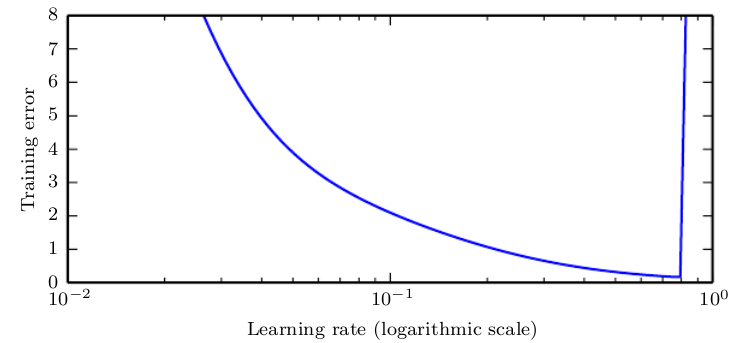
\includegraphics[width=6in]{fig/chap11/11_1.png} 
   \caption{学习率和训练误差之间的典型关系。 可以看到当学习高于一个最佳值时误差急剧上升。 这里的训练时间是固定的,因为较小的学习率有时可能仅仅减慢了训练,且减慢的速度和学习率减小量成比例。 泛化误差可以遵循该曲线,或者由于具有过大或过小的学习率而引起的正则化效应而变得复杂,因为较差的优化可以在一定程度上减少或防止过拟合,并且甚至在等效的训练误差下具有不同的泛化误差。}
   \label{fig:11_1}
\end{figure}

调整学习率以外的参数需要同时监控训练误差和测试误差,以诊断您的模型是过度拟合还是欠拟合,然后适当调整其容量。

如果你在训练集上的错误率高于你的目标错误率,除了增加模型容量没有别的选择。如果你不使用正则化,并且你确信自己的优化算法正确地执行了,则必须向网络中添加更多层或添加更多隐藏单元。但这增加了模型的计算成本。

如果你在测试集上的错误率高于目标错误率,您可以采取两种操作。测试误差是训练误差和训练与测试误差之间差距的和。 通过权衡这些量可以找到最佳测试误差。 神经网络通常在训练误差非常低(则容量高时)时表现得最好,并且测试误差主要由其与训练误差之间的差距来驱动。 你的目标是快速地减少这个差距,而并不增加训练误差。 为了减少这个差距,你要改变用于正则化的超参,以减少有效模型容量,例如添加dropout或权重衰减。 最佳的性能往往来自于大模型,而且它是较好地正则化的,如使用dropout。

大多数超参可以通过推断它们是增加还是降低模型容量和设置,一些例子如表\ref{tab:11.1}所示。

\begin{table}[!hbp]
    \begin{tabular}{|c|c|c|c|}
        \hline
        \hline
        超参 & 何时可使增大容量 & 原因 & 注意点 \\
        \hline
        隐藏单元数量 & 增加 & 增加隐藏单元数量可以增加模型的表达能力 & 增加隐藏单元数量会对模型的每个操作都增加计算和内存消耗 \\
        \hline
        学习率 & 调整到最优 & 一个过大或过小的不当的学习率会导致优化失败而使得模型有效容量低 & \\
        \hline
        卷积核宽度 & 增大 & 增大卷积核宽度会增加模型的参数个数 & 较宽核的输出较窄,除非使用0填充来减小影响,否则会降低模型容量。宽核需要更多的内存来存储参数,并且计算量增加,但更窄的输出可以减少内存消耗。 \\
        \hline
        隐式0填充 & 增加 & 在卷积前加入隐式0填充可以保持较大的表达尺寸 & 对于大部分的操作都增加了时间和内容的消耗 \\
        \hline
        权重衰减系数 & 减小 & 减小权重衰减系数会让模型的参数自由而变大 &  \\
        \hline
        Dropout比例 & 减小 & Dropout单元会减少各个单元之间“合作”的机会来拟合训练集 &  \\
        \hline
        \hline
    \end{tabular}
    \caption{各种超参对模型容量的影响}
    \label{tab:11.1}
\end{table}

在手动调整超参时,不要忽视你的最终目标,即在测试集上获得良好的性能。添加正则化只是实现这一目标的一种方法。只要你具有低的训练误差,你始终可以通过收集更多的训练数据来减少泛化误差。实际中保证成功的一个暴力的方法是不断增加模型容量和训练集大小,直到任务被解决。这种方法必然增加了训练和预测的计算成本,因此只有在适当的资源下才是可行的。 理论上这种方法可能由于优化困难而失败,但对于许多问题,只要选择合适的模型,优化似乎不是重要的障碍。


\subsection{自动超参优化算法}
理想的学习算法只需要一个数据集然后输出一个函数,而不需要手动调节超参。一些比较受欢迎的算法,如逻辑回归和SVM源于它们本身的能力,只调节用一、两个超参就可获得良好效果。 神经网络有时可以只调节少数的超参而表现不错,但是通常需要调节四十个或更多个的超参来获得大幅度的提升。 对于手动调整超参,当使用者有一个良好的起始条件,例如重用了别人的类似的应用和架构,或者当使用者具有类似任务的数月或多年的超参探索经验时可以获得较好的效果。 然而,对于大部分应用,往往没有这样的起始条件。在这些情况下,自动算法可以找到有效的超参值。

当我们考虑一个学习算法使用者在搜索一个好的超参时所使用的方式,意识到这正是在进行优化:即我们试图找到超参的值来优化目标函数,例如验证误差,而且有时它是被一定条件约束的(例如训练耗时、内存消耗或识别耗时)。因此,理论上我们可以开发一个学习算法的选择超参的优化算法,从而将超参对使用者进行隐藏。不幸的是,超参优化算法通常有它们自己的超参,例如每个学习算法的超参应该有取之范围。然而,这些辅助超往往更容易选择, 某种意义上,使用同样辅助超参的任务中的大部分可以获得可接受的效果。

